\documentclass[reprint,english,notitlepage]{revtex4-1}  % defines the basic parameters of the document

% if you want a single-column, remove reprint

% allows special characters (including æøå)
\usepackage[utf8]{inputenc}
\usepackage[english]{babel}
\usepackage{comment}

%% note that you may need to download some of these packages manually, it depends on your setup.
%% I recommend downloading TeXMaker, because it includes a large library of the most common packages.

\usepackage{physics,amssymb}  % mathematical symbols (physics imports amsmath)
\usepackage{graphicx}         % include graphics such as plots
\usepackage{xcolor}           % set colors
\usepackage{hyperref}         % automagic cross-referencing (this is GODLIKE)
\usepackage{tikz}             % draw figures manually
\usepackage{listings}         % display code
\usepackage{subfigure}        % imports a lot of cool and useful figure commands

% defines the color of hyperref objects
% Blending two colors:  blue!80!black  =  80% blue and 20% black
\hypersetup{ % this is just my personal choice, feel free to change things
    colorlinks,
    linkcolor={red!50!black},
    citecolor={blue!50!black},
    urlcolor={blue!80!black}}

%% Defines the style of the programming listing
%% This is actually my personal template, go ahead and change stuff if you want
\lstset{ %
	inputpath=,
	backgroundcolor=\color{white!88!black},
	basicstyle={\ttfamily\scriptsize},
	commentstyle=\color{magenta},
	language=Python,
	morekeywords={True,False},
	tabsize=4,
	stringstyle=\color{green!55!black},
	frame=single,
	keywordstyle=\color{blue},
	showstringspaces=false,
	columns=fullflexible,
	keepspaces=true}


%% USEFUL LINKS:
%%
%%   UiO LaTeX guides:        https://www.mn.uio.no/ifi/tjenester/it/hjelp/latex/ 
%%   mathematics:             https://en.wikibooks.org/wiki/LaTeX/Mathematics

%%   PHYSICS !                https://mirror.hmc.edu/ctan/macros/latex/contrib/physics/physics.pdf

%%   the basics of Tikz:       https://en.wikibooks.org/wiki/LaTeX/PGF/TikZ
%%   all the colors!:          https://en.wikibooks.org/wiki/LaTeX/Colors
%%   how to draw tables:       https://en.wikibooks.org/wiki/LaTeX/Tables
%%   code listing styles:      https://en.wikibooks.org/wiki/LaTeX/Source_Code_Listings
%%   \includegraphics          https://en.wikibooks.org/wiki/LaTeX/Importing_Graphics
%%   learn more about figures  https://en.wikibooks.org/wiki/LaTeX/Floats,_Figures_and_Captions
%%   automagic bibliography:   https://en.wikibooks.org/wiki/LaTeX/Bibliography_Management  (this one is kinda difficult the first time)
%%   REVTeX Guide:             http://www.physics.csbsju.edu/370/papers/Journal_Style_Manuals/auguide4-1.pdf
%%
%%   (this document is of class "revtex4-1", the REVTeX Guide explains how the class works)


%% CREATING THE .pdf FILE USING LINUX IN THE TERMINAL
%% 
%% [terminal]$ pdflatex template.tex
%%
%% Run the command twice, always.
%% If you want to use \footnote, you need to run these commands (IN THIS SPECIFIC ORDER)
%% 
%% [terminal]$ pdflatex template.tex
%% [terminal]$ bibtex template
%% [terminal]$ pdflatex template.tex
%% [terminal]$ pdflatex template.tex
%%
%% Don't ask me why, I don't know.

\begin{document}
\title{This is a Very Important Title!}   % self-explanatory
\author{Person McSomething}               % self-explanatory
\date{\today}                             % self-explanatory
\noaffiliation                            % ignore this
\begin{abstract}                          % marks the beginning of the abstract
This abstract is abstract.                % the body of the abstract
\end{abstract}                            % marks the end of the abstract
\maketitle                                % creates the title, author, date & abstract


% the fundamental components of scientific reports:
\section{Introduction}






\section{Conclusion}
Assumptions: const V, P, N.



%% When it comes to the bibliography I personally generate it using BibLaTeX. (see the link above if you're interested)
%% You're obviously allowed to create the references section however you like.
%% I'll keep it simple here.
\section*{References}  % the asterisk (*) after \section makes the section numbering go away
\begin{itemize}
\item[-]Reference 1
\item[-]Reference 2
\end{itemize}

\newpage
%% if you want to include an appendix, this is how you do it
\appendix
\section*{Appendix I.}

In figure \ref{fig:mugs} we can see the temperature of the Temperfect mug and the Bodum mug plotted against the time. Since the water was not poured at the same temperature this has been adjusted in the plot as seen in figure \ref{fig:mugs_2}. 

We can see from figure \ref{fig:mugs} that the Temperfect mug absorbs a lot of heat very quickly. This is because it goes trough a phase change, from solid to liquid. It then slowly goes back to solid again and gives heat back to the liquid in the mug. That makes it so that the temperature of the liquid drops more slowly. When all of the material in the mug is solid, the liquid will drop in temperature as if it was a regular mug, like the Bodum.

The reason this is beneficial is that the heat flux is related to the $\nabla T$, so by reducing the temperature quickly, and storing it as latent heat, you can re-introduce it to the liquid later, at a lower temperature and therefore reduce the heat flux.



\begin{figure}
\centering
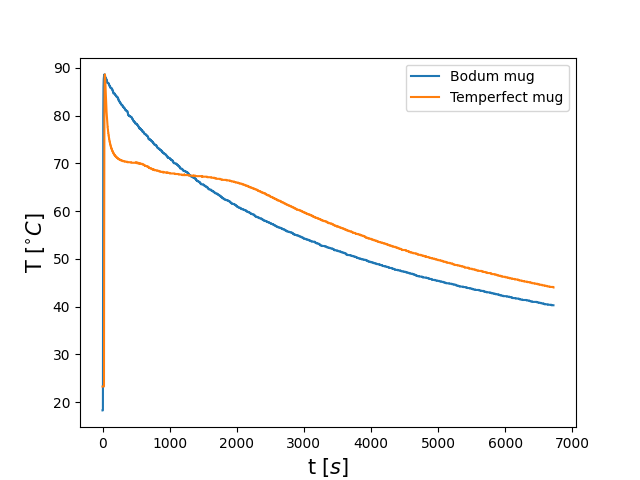
\includegraphics[width=8cm]{../figures/mugs.png}
\caption{Temperature against time for the two mugs.}
\label{fig:mugs}
\end{figure}

\begin{figure}
\centering
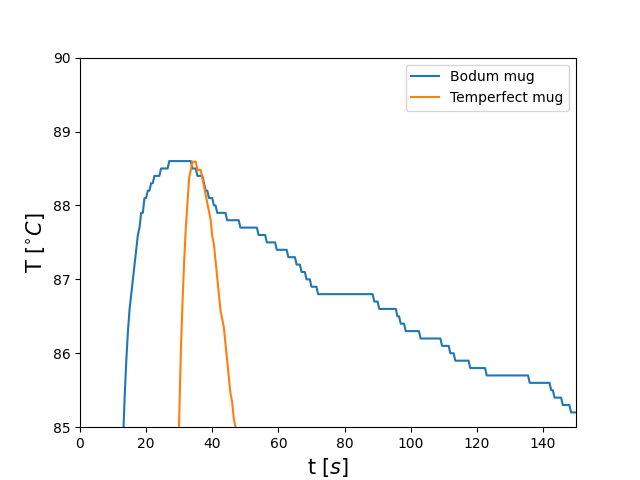
\includegraphics[width=8cm]{../figures/mugs_2.png}
\caption{Closeup of the starting points where the hot water is poured in.}
\label{fig:mugs_2}
\end{figure}



Assume constant pressure $P$ and volume $V$. This means that the work $W=0$, so that the change in internal energy $dU=dQ$. We also assume a constant number of particles $N$. In this condition we can use the definition of temperature(given by the total differential of the entropy $S$), so that the temperature $T$ is given by

$$T^{-1}=(\frac{\partial S}{\partial U})_{N,V},$$
Since we only have that $S$ is a function of $T$ we get that 
$$
T^{-1}=\frac{d S}{d U}= \frac{dS}{dQ} =\frac{d S}{dT}\frac{d T}{d Q}.
$$

$$ T^{-1}\frac{dQ}{dT}=\frac{dS}{dT}.$$

Under constant volume the heat capacity $C_V=(\partial U/\partial T)_{V,N}$, that becomes $C_V=(dQ/dT)$ in our case. We then get that 
\begin{equation}\label{}
\frac{dS}{dT}=\frac{C_V}{T}.
\end{equation}


In figure \ref{fig:dSdT_mot_T} we see the slope of the entropy $dS/dT$ against the temperature $T$, calculated by this method in H2O. The heat capacity of H2O is listed in \ref{table:h2o}. We use this to calculate the entropy. In figure \ref{fig:S_mot_T} we see the entropy against the temperature.

\begin{table}[h]  % h = "here"  , h! = here!
\caption{Table of the heat capacity $C$ of H2O in $kJ/kgK$.}\label{table:h2o}
\begin{tabular}{|c|c|} % note that & separates columns while \\ separates the rows
\hline                    % creates a horizontal line (try removing it)
Solid & $2.108$  \\
\hline
Liquid & $4.184$ \\
\hline
Gas & $1.996$ \\
\hline
\end{tabular}
\end{table}


\begin{figure}
\centering
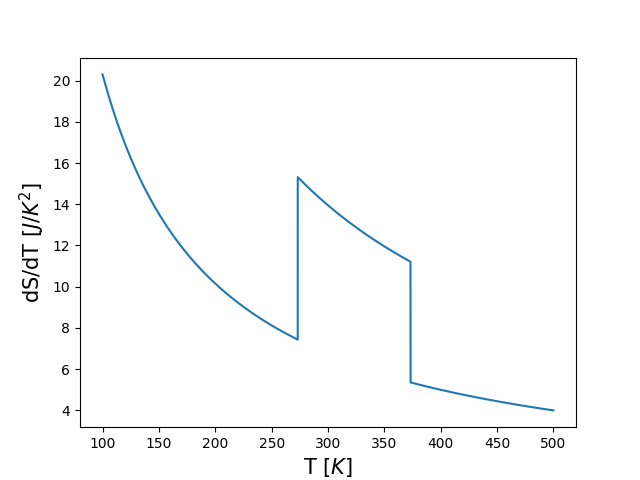
\includegraphics[width=8cm]{../figures/dSdT_mot_T.png}
\caption{Figure of the slope of entropy $dS/dT$ against the temperature $T$.}
\label{fig:dSdT_mot_T}
\end{figure}

\begin{figure}
\centering
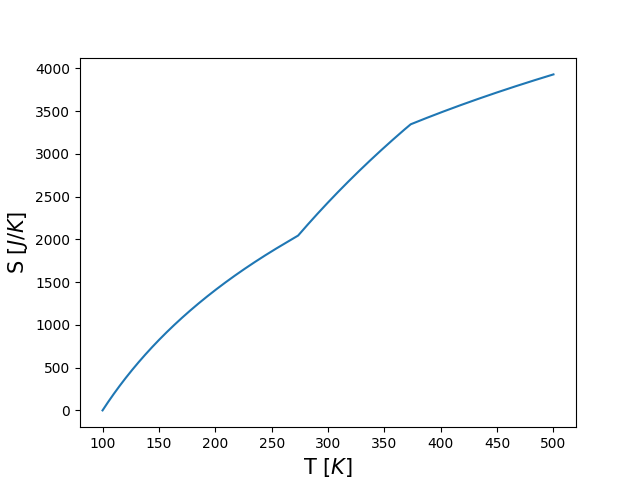
\includegraphics[width=8cm]{../figures/S_mot_T.png}
\caption{Figure of the entropy $S$ against the temperature $T$.}
\label{fig:S_mot_T}
\end{figure}



The feature of the graph that is relevant is the part where the phase changes are happening. That is from ca. $0$s to $2000$s.

\section*{Appendix II.}
\subsection*{A.}
The multiplicity of an Einstein crystal is given by 
$$ \Omega(N,q)\approx \frac{(q+N)!}{q!N!},$$
 where $q$ is the number of energy units $\epsilon=hf$, where $f$ is the frequency and $h$ is Planck's constant, and $N$ is the number of particles in the crystal. We use this to find the entropy
  $$S=k\ln\Omega,$$ 
  where $k$ is Boltzmann's constant. We have that the internal energy of the crystal is 
  $$U=q\epsilon+\frac{N}{2}\epsilon,$$
  if we include the ground-states. This of course gives us that 
  $$ dU=\epsilon dq,$$
  since we vary $q$. 
  
  The thermodynamic identity says that 
  $$ dU=TdS-PdV+\mu dN,$$
  where $\mu$ is the chemical potential, $P$ is the pressure and $V$ is the volume. We assume that the volume, pressure and number of particles stay constant. We then get that
  $$T= \frac{dU}{dS}=\epsilon\frac{dq}{dS}\Leftrightarrow \frac{T}{\epsilon}=\frac{dq}{dS}.$$
  Numerically we find this as
  $$\tilde{T_i} =\frac{T_i}{\epsilon}=\frac{q_i-q_{i-1}}{S_i-S_{i-1}}.$$

We have that the heat capacity 
$$C_V=\frac{dU}{dT}=\epsilon\frac{dq}{dT}=\frac{dq}{dT/\epsilon}=\frac{dq}{d\tilde{T}}.$$
We find this numerically as 
$$ C_{V,i}=\frac{q_{i}-q_{i-1}}{\tilde{T}_i-\tilde{T}_{i-1}}.$$

\begin{figure}
\centering
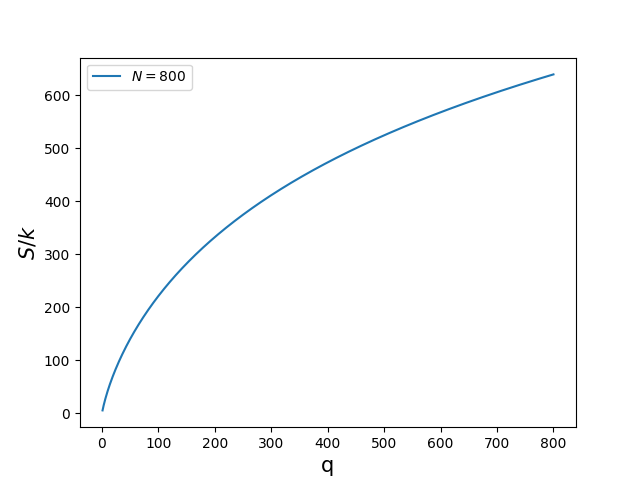
\includegraphics[width=8cm]{../figures/S_mot_q.png}
\caption{Figure of numerically calculated entropy $S/k$ against the number of energy units $q$.}
\label{fig:S_mot_q}
\end{figure}
  
\begin{figure}
\centering
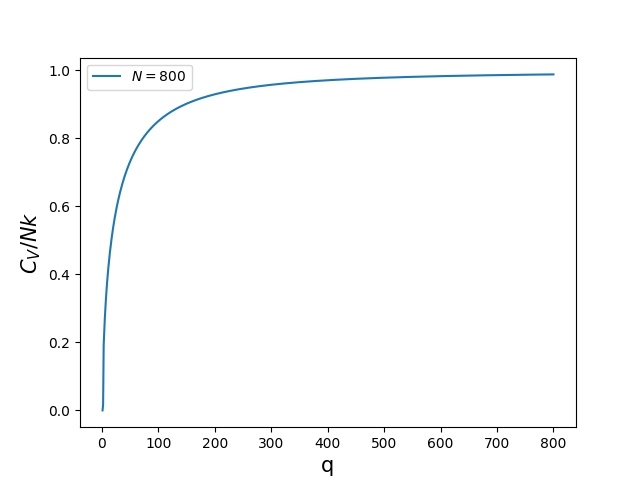
\includegraphics[width=8cm]{../figures/C_mot_q.png}
\caption{Figure of numerically calculated heat capacity $C_V$ against the number of energy units $q$.}
\label{fig:C_mot_q}
\end{figure}

We see $S/k$ as a function of $q$ in figure \ref{fig:S_mot_q} and $\frac{C_V}{Nk}$ as a function of $q$ in figure \ref{fig:C_mot_q}.

\subsection*{B.}

We have that the multiplicity of an Einstein solid is $$\Omega(N,q)=\frac{(q+N-1)!}{q!(N-1)!},$$
where $N$ is the number of particles and $q$ is the number of energy units $\hbar f$. If we use $N>>1$, we can see that $$ \Omega(N,q)\approx \frac{(q+N)!}{q!N!}.$$

If also have $q>>1$ we can Stirling approximate this expression. That means that the temperature is $T>0K$. This gives us that
$$ \Omega = \frac{(q+N)!}{q!N!}\approx\frac{(q+N)^{q+N} e^{-(q+N)}}{q^q e^{-q} N^N e^{-N}}=(\frac{q+N}{q})^q(\frac{q+N}{N})^N$$ 
\\~\\
From the lectures we have that the multiplicity for the low temperature limit is $$\Omega_{low\ T}(q,N)\approx (\frac{Ne}{q})^q.$$
And the high temperature limit is $$ \Omega_{high\ T}\approx (\frac{qe}{N})^N.$$

\begin{figure}
\centering
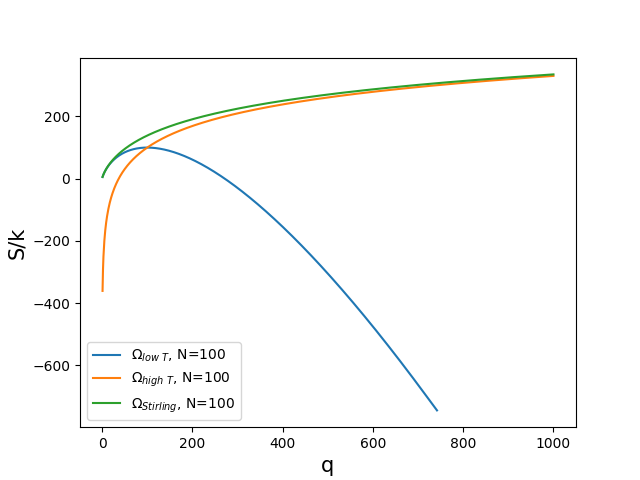
\includegraphics[width=8cm]{../figures/omegas.png}
\caption{Figure of the low temperature approximation of the multiplicity $\Omega_{low\ T}$ vs. the high temperature approximation $\Omega_{high\ T}$ vs. the Stirling approximation $\Omega_{Stirling}$ against the number of energy units $q$.}
\label{fig:omegas}
\end{figure}

We see the comparison of the different $\Omega$'s against each other in figure \ref{fig:omegas}. From the figure we see that the low temperature approximation fits the Stirling approximation at low $q$ and the high temperature approximation at high $q$.

~\\
We had that $$dS=\frac{1}{U/Nk}dU=\frac{Nk}{U}dU=\frac{2Nk}{2q+N}dq.$$

This gives us that the entropy is $$S(U,N)=Nk\int_{U_0}^U \frac{1}{U}dU=Nk ln\frac{U}{U_0},$$

where $U_0=(1/2)N\epsilon$ is the ground state energy.
~\\

 We have that the temperature $$T(U,N)=(\frac{\partial S}{\partial U})^{-1}=(Nk\frac{1}{U})^{-1}=\frac{U}{Nk}.$$
 ~\\
 And that the heat capacity $$C_V(T,N)=\frac{dU}{dT}=\frac{d}{dT}(NkT)=Nk.$$

The specific heat capacity per. mole is $$ c=\frac{C}{n}=\frac{Nk}{n},$$
where $n=N/N_A$ is the number of moles and $N_A$ is Avogadro's number. We then get that 
$$ c=\frac{Nk}{N/N_A}=N_Ak=R,$$
where $R$ is the universal gas constant.

\subsection*{C.}
We see from figure \ref{fig:C_mot_q} that $C_V/Nk$ goes to one. This means that our analytical and numerical results corresponds more and more as $q$ gets higher. 

COMPARE TO FIG 1.14 CMON COMPARE NOW!!!! COMPAAAAARE!!!!!!!

\section*{APPENDIX III.}
Since we have that 
$$U=NkT=\epsilon q+\frac{N}{2}\epsilon$$ 
for the Einstein crystal, we can see that
$$ dU=NkdT=\epsilon dq\Leftrightarrow dT=\frac{\epsilon}{Nk}dq.$$
We can use this to model how $q$ changes in the mug, changes the temperature of the mug material. But the Einstein solid is not valid for liquids. The Temperfect mug has a material that will melt when you put hot liquid in the mug and therefore the Einstein model is not valid at that point. After a period of time the mug material will go back into solid and here the Einstein model might be valid. As energy units is transferred from the mug material to the liquid in the mug. 

%% all \section commands following \appendix are automatically taken as appendices

%% Note that \label{appendix} command on line 115. What this does is setup a reference point for LaTeX that you can
%% access wherever you want using \ref{appendix}.
%% You can place labels on most environments such as equations, figures, tables, etc.


%% If you want to include figure:
%\includegraphics[scale=1.0]{filename}
%% check https://en.wikibooks.org/wiki/LaTeX/Importing_Graphics if you want to know more

\end{document}
